
% Template for HC2 documents
% 
% Please create a different file for each language
%
% Dependencies:
% - This file should compile if you have installed all the LaTeX extensions
%   (texlive-full in Ubuntu)
% - You will need the program "hevea" to convert to HTML
%
% Caveats:
% - Please use the "verbatim" environment for code, and please use spaces instead of tabs
% - Hevea does not convert the images properly, however this can be done manually
%   (you just need to convert the pictures to PNG and rename your pictures  hc2template001.png
%   etc.) We will anyway have to do some magic with the HTML files so that they work
%   in Mooshak
% - Please use only $ and $$ for math environments, and never \begin{equation}
\documentclass[11pt,a4paper]{article}
\usepackage{mathptmx}
\usepackage[in]{fullpage}
\usepackage[absolute]{textpos}
\usepackage{graphicx}
\usepackage[ngerman]{babel}
\usepackage[utf8]{inputenc}
\usepackage{fancyhdr}
\usepackage{moreverb}
\usepackage{color}
\usepackage{url}
\usepackage{longtable}
\pagestyle{fancy}

\definecolor{gray}{RGB}{128,128,128}

\renewcommand{\baselinestretch}{0.92}

%%%%%%%%%%%%%%%%%%%%%%%%%%%%%%%%%%%%%%%%%%%%%%%%%%%%%%%%%%%%%%%%%%%%%%%%%%%%%%%%%%%%%%%%%

% Put the title of your document here
\newcommand{\titleinfolong}{Teamhandbuch für den Helvetic Coding Contest 2015}
\newcommand{\titleinfo}{Teamhandbuch}
% Put the author of the document here
\newcommand{\authorinfo}{Robert R.~Enderlein}
% Put the language of the document here
\newcommand{\langinfo}{Deutsch}
% Put the name of the Task (or some short identifying information of the document) here
\newcommand{\taskinfo}{Teamhandbuch}

%%%%%%%%%%%%%%%%%%%%%%%%%%%%%%%%%%%%%%%%%%%%%%%%%%%%%%%%%%%%%%%%%%%%%%%%%%%%%%%%%%%%%%%%%


\title{\titleinfolong}
\author{von \authorinfo\footnote{Dieses Handbuch basiert auf dem Teamhandbuch von
Domjudge.}}
\date{}

\renewcommand{\headrulewidth}{0pt}
\renewcommand{\footrulewidth}{0.4pt}
\lhead{}
\chead{}
\rhead{}
\lfoot{\textcolor{gray}{Helvetic Coding Contest 2015}}
\cfoot{\thepage}
\rfoot{\textcolor{gray}{\titleinfo}}

\begin{document}
\maketitle
\thispagestyle{fancy}
\setcounter{page}{1} 

%\begin{latexonly}
\begin{textblock*}{20mm}(170mm, 15mm)

\includegraphics[width=20mm]{hc2logogray.pdf}
\end{textblock*}

\begin{textblock*}{50mm}(25.4mm, 25.4mm)
\noindent \textcolor{gray}{\langinfo \\ \textbf{\taskinfo} }
\end{textblock*}
%\end{latexonly}

%%%%%%%%%%%%%%%%%%%%%%%%%%%%%%%%%%%%%%%%%%%%%%%%%%%%%%%%%%%%%%%%%%%%%%%%%%%%%%%%%%%%%%%%%
%%%%%%%%%%%%%%%%%%%%%%%%%%%%%%%%%%%%%%%%%%%%%%%%%%%%%%%%%%%%%%%%%%%%%%%%%%%%%%%%%%%%%%%%%
%%%%%%%%%%%%%%%%%%%%%%%%%%%%%%%%%%%%%%%%%%%%%%%%%%%%%%%%%%%%%%%%%%%%%%%%%%%%%%%%%%%%%%%%%
% Start here

% There is a bug in the hevea package. The following construct will make sure
% that everything written in \heaveaonly will be written only in Hevea
% htmlonly doesn't work for some reason
\newcommand{\heveaonly}[1]{#1}
%\begin{latexonly}
\renewcommand{\heveaonly}[1]{}
%\end{latexonly}

\noindent Die folgenden Informationen sind eine Kurzzusammenfassung des
Wettbewerb-Systems. Sie soll als Einführung dienen, so dass ihr das System von
Beginn an verwenden könnt. Wir empfehlen aber, dass mindestens ein Teammitglied
das ganze Handbuch durchliest. Einige Details können wichtig werden, falls
Probleme auftauchen.

Domjudge verfügt über ein Webinterface unter folgender Adresse:
\url{https://ec2.hc2.ch/team}.
Die Abbildungen \ref{fig:overview}, \ref{fig:statements}, \ref{fig:ranking}
geben einen ersten Eindruck der Oberfläche.

\begin{figure*}[t]
\begin{center}
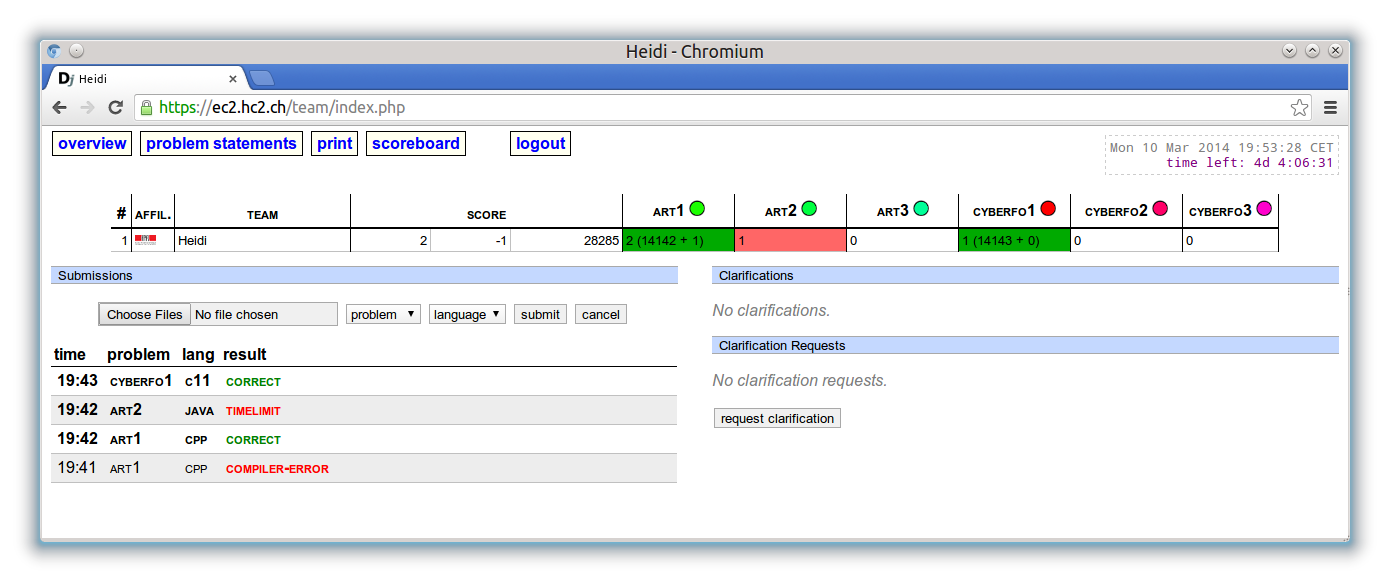
\includegraphics[width=0.73\textwidth]{overview.png}
\end{center}
\vskip -2 em
\caption{Die Übersichtsseite für Teams.}
\label{fig:overview}

\begin{center}
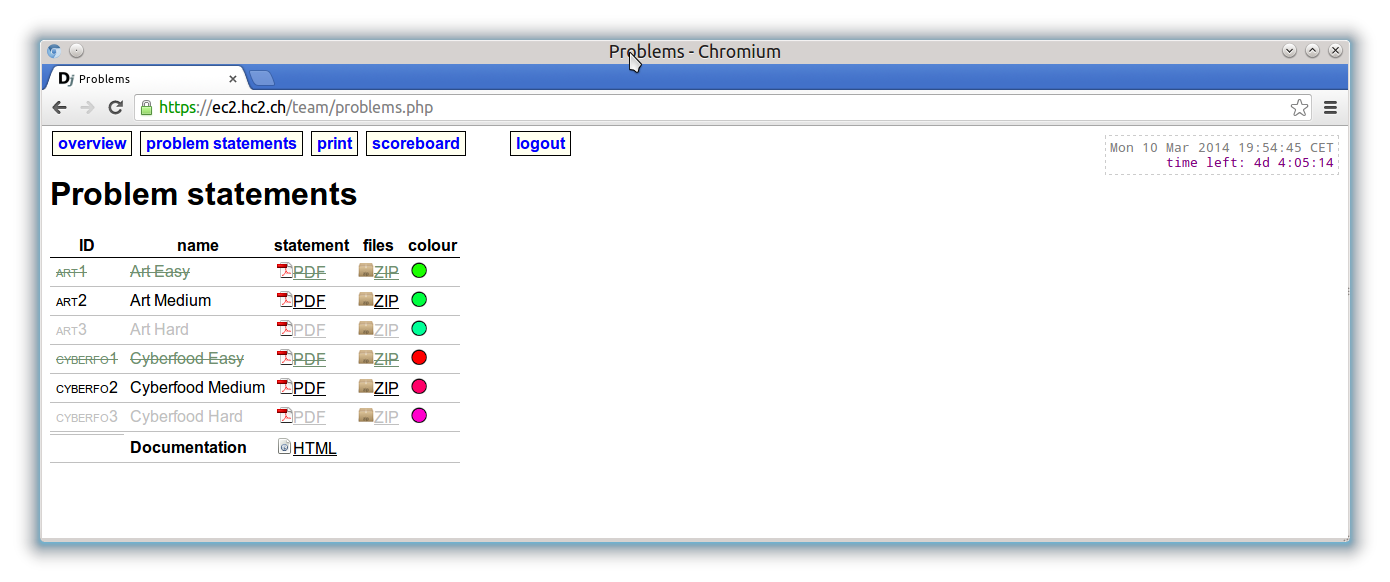
\includegraphics[width=0.73\textwidth]{statements.png}
\end{center}
\vskip -2 em
\caption{Die Seite mit den Aufgabenstellungen.}
\label{fig:statements}

\begin{center}
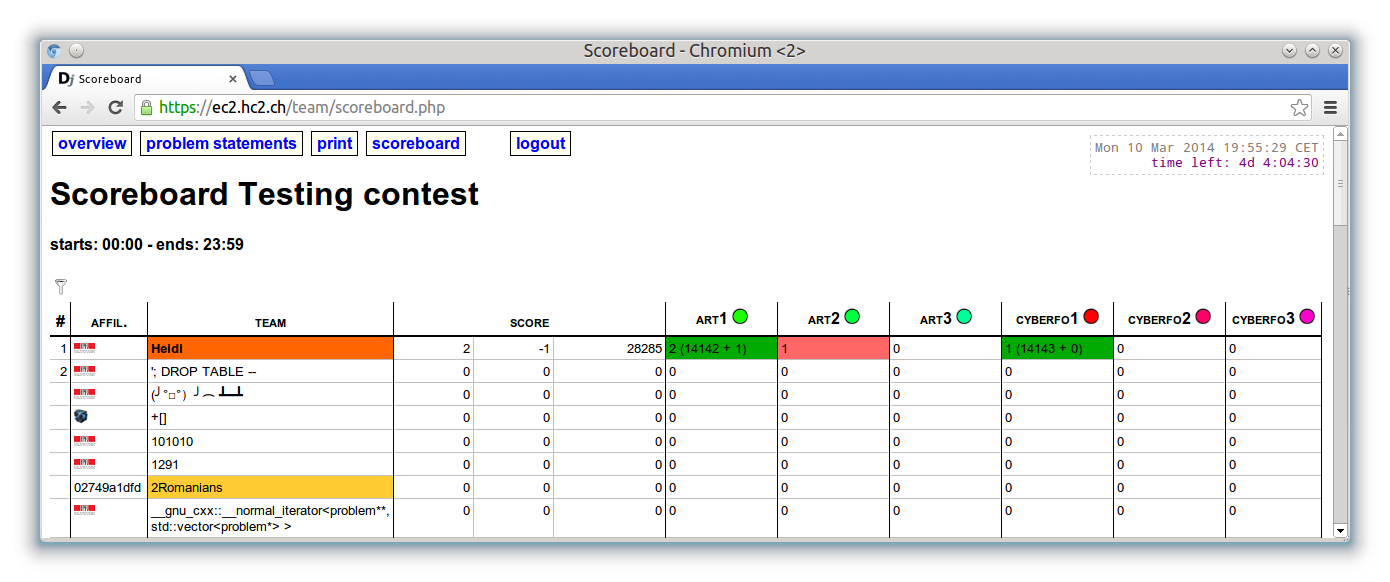
\includegraphics[width=0.73\textwidth]{ranking.png}
\end{center}
\vskip -2 em
\caption{Die Rangliste.}
\label{fig:ranking}
\end{figure*}

\paragraph{Aufgabenstellungen und zusätzliches Material.}
Die Aufgabenstellungen und weitere Dateien sind unter dem Link \glqq Problem
statements\grqq{} auf eurer Teamseite zugänglich. Einige Aufgabenstellungen sind
zunächst deaktiviert; ihr könnt sie erst ansehen, wenn ihr die Aufgabe darüber
gelöst habt.
Siehe Abbildung~\ref{fig:statements}.

\paragraph{Lesen und schreiben.}
Eure Lösung muss die Aufgabenstellung von der Standardeingabe (\glqq standard in\grqq{})
lesen, und die Antwort in die Standardausgabe (\glqq standard out\grqq{}) schreiben.
Keine (anderen) Dateien müssen geöffnet werden.
Siehe Sektion~\ref{codeexamples} für Beispielquellcode.
Falls ihr Java benützt, denkt daran, dass java.util.Scanner für grosse
Aufgaben zu langsam ist.

Java, Scala: bleibt bitte im default Package, i.e., verwendet bitte keine \texttt{package} Direktive.

\paragraph{Lösungen kompilieren und testen.}
Verwendet die folgenden Befehle, um eure Lösungen zu kompilieren und testen (ersetzt die
\textbf{fett} gedruckten Teile).
\begin{center}
\begin{tabular}{l|p{5cm}|p{7cm}}
C&hc2-compile \textbf{prob1}.c &hc2-run \textbf{prob1}.c $<$ \textbf{01}.in\\
C++11&hc2-compile \textbf{prob1}.cpp &hc2-run \textbf{prob1}.cpp $<$ \textbf{01}.in\\
C++98&hc2-compile \textbf{prob1}.c98 &hc2-run \textbf{prob1}.c98 $<$ \textbf{01}.in\\
Java&hc2-compile \textbf{Prob1}.java &hc2-run \textbf{Prob1}.java $<$ \textbf{01}.in\\
Scala&hc2-compile \textbf{Prob1}.scala &hc2-run \textbf{Prob1}.scala $<$ \textbf{01}.in\\
Python 2&hc2-compile \textbf{prob1}.py &hc2-run \textbf{prob1}.py $<$ \textbf{01}.in\\
Python 3&hc2-compile \textbf{prob1}.py3 &hc2-run \textbf{prob1}.py3 $<$ \textbf{01}.in\\
Ruby&hc2-compile \textbf{prob1}.rb &hc2-run \textbf{prob1}.rb $<$ \textbf{01}.in\\
Text&hc2-compile \textbf{prob1}.txt &hc2-run \textbf{prob1}.txt $<$ \textbf{01}.in\\
\end{tabular}
\end{center}

\paragraph{Lösungen einsenden.}
Begebt euch auf die Übersichtsseite (\glqq Overview\grqq{},
\url{https://ec2.hc2.ch/team}).
Klickt auf \glqq Select file...\grqq{} in der linken Spalte. Wählt die Datei,
welche ihr einsenden wollt. Die Aufgabe und Programmiersprache werden
automatisch anhand des Dateinamens erkannt. Siehe auch
Abbildung~\ref{fig:overview}.

\paragraph{Drucken.}
Unter den Link \glqq{} print \grqq{} auf eurer Teamseite,
erreicht ihr ein Formular wo ihr Dateien drucken lassen könnt.
Wir werden euch das Dokument an euren Platz liefern. \emph{Bitte holt es nicht
selbst ab.} Der Umwelt zuliebe bitten wir euch, das Drucken mit Zurückhaltung zu
geniessen.


\clearpage
\section{Lösungen einsenden}
\label{sec:submit}
Lösungen werden über das Webinterface von Domjudge eingereicht, unter
\url{https://ec2.hc2.ch/team}. Beim ersten Besuch müsst ihr euch mit eurem
Benutzernamen und Passwort einloggen (diese werden euch kurz vor Beginn des
Wettbewerbs verteilt). Bei Problemen bitten wir euch, die Hand zu heben. Ein
Organisator wird kommen, um euch zu helfen.

Klickt in der linken Spalte auf \glqq Select file...\grqq{}, um eine Datei zum
einsenden auszuwählen. Domjudge versucht, die Aufgabe und Programmiersprache vom
Namen der Datei und ihrer Endung zu erkennen. Falls das nicht klappt, wählt dies
bitte selbst aus.

Nachdem ihr auf \glqq submit\grqq{} geklickt habt und eure Abgabe bestätigt
habt, werdet ihr zur Liste der Abgaben weitergeleitet. Dort seht ihr eine
Nachricht, dass eure Abgabe erfolgreich war. Eure Lösung sollte in der Liste
vorhanden sein. Falls etwas schief gelaufen ist, informiert euch eine
Fehlermeldung über das Problem.

\section{Resultate eurer Einsendungen ansehen}
Die linke Spalte der Teamseite zeigt euch eine Übersicht über alle Lösungen, die
ihr eingesandt habt. Sie enthält die Zeit der Abgabe, die Programmiersprache,
die Aufgabe und der Status der Abgabe. Ihr findet eure Teamseite auf
\url{https://ec2.hc2.ch/team}.

Oben an der Seite seht ihr euren Eintrag in der Rangliste: euren aktuellen Rang
und welche Aufgaben ihr schon versucht resp.\ gelöst habt. Über das Menu könnt
ihr die gesamte Rangliste mit allen Teams sehen. Diese Rangliste wird eine
Stunde vor Wettbewerbsende \glqq eingefroren\grqq{} und nicht mehr aktualisiert.
Der Eintrag auf eurer Teamseite wird zwar noch aktualisiert, aber ihr seht dort
\glqq ?\grqq{} als Rang.

\subsection{Mögliche Resultate}
Eine eingesandte Lösung kann zu folgenden Resultaten führen:

\begin{center}
\begin{longtable}{|l|p{12.5cm}|}
\hline
\textbf{Bewertung} &
\textbf{Beschreibung}\\\hline
Correct &
Euer Programm hat alle Testfälle bestanden: Ihr habt die Aufgabe gelöst!\\\hline
Compiler-error &
Beim Kompilieren eures Programms ist ein Fehler aufgetreten. Auf der Detailseite
der Abgabe könnt ihr die genaue Fehlermeldung sehen.
\\\hline
Timelimit &
Euer Programm überschritt das Zeitlimit und wurde abgebrochen. Möglicherweise
bleibt euer Programm in einer Schleife hängen, oder eure Lösung ist nicht
effizient genug.\\\hline
Run-error &
% FIXME: exit code 0 is rather irrelevant for hc2, isn't it?
Beim Ausführen eures Programms ist ein Fehler aufgetreten. Dies kann
verschiedene Ursachen haben, z.\,B. Division durch Null, ungültige
Speicherzugriffe (wie etwa zu grosse Array-Indizes), das Benützen von
zuviel Speicher etc. Überprüft auch, ob euer Programm den Rückgabewert 0
zurück gibt!\\\hline
No-output&
Euer Program produzierte keine Ausgabe. Möglicherweise hat sich euer
Programm vorzeitig beendet.\\\hline
Wrong-answer&
Eure Antwort war falsch. (Der Jury ignoriert Unterschiede in Leerzeichen.)
\\\hline
Too-late&
Sorry, ihr wart zu spät, der Wettbewerb ist bereits vorbei. Eure Lösung kann
nicht mehr ausgewertet werden.\\\hline
\end{longtable}
\end{center}

\bigskip

\section{Klarstellungen}
Jegliche Kommunikation mit der Jury funktioniert über Klarstellungen. Diese
findet ihr in der rechten Spalte eurer Teamseite. Sowohl Antworten der Jury als
auch eure Anfragen werden dort angezeigt.

Es hat ebenfalls einen Knopf \glqq request clarification\grqq{}, mit dem ihr
eine Anfrage an die Jury stellen könnt. Diese Anfrage ist nur für die Jury
lesbar. Sie wird sobald als möglich beantwortet. Antworten, welche für alle
Teams relevant sind, werden an alle Teilnehmer geschickt.

Ihr seid selbst dafür verantwortlich, regelmässig nach den Klarstellungen zu
sehen!

\section[Bewertung]{Wie werden Lösungen bewertet?}
\subsection{Lösungen einsenden}
Eure Lösungen werden mittels des Webinterfaces eingereicht (Siehe Kapitel
\ref{sec:submit}). Beachtet, dass ihr den Quellcode eures Programms einreicht,
und nicht das kompilierte Programm oder die Ausgabe (ausser die Aufgabenstellung
verlangt explizit nach einer Textdatei). Nach dem Einsenden gelangt
eurer Programm in eine Warteschlange, wo es darauf wartet, auf einem
Jurycomputer kompiliert, ausgeführt und getestet zu werden.

\subsection{Kompilation}
Euer Programm wird auf einem Juryrechner kompiliert. Dieser läuft unter Ubuntu
Linux (64 bits).

Folgende Befehle werden zum Kompilieren verwendet:
\begin{center}
\begin{tabular}{l|p{14cm}}
C&
gcc -Wall -O2 -static -pipe -o \$DEST \$SOURCE -lm \\
C++11&
g++ -Wall -O2 -static -pipe -std=c++11 -o \$DEST -x c++ \$SOURCE \\
C++98&
g++ -Wall -O2 -static -pipe -o \$DEST -x c++ \$SOURCE \\
Java&
javac -d . \$SOURCE \\
Scala&
scalac \$SOURCE \\
Ruby&
ruby -c \$SOURCE \\
\end{tabular}
\end{center}
In diesen Befehlen steht \$SOURCE für den Namen eurer Datei.
Python Quellcode und Textdateien werden nicht kompiliert.

\subsection{Testphase}
Sobald euer Programm erfolgreich kompiliert ist, wird es ausgeführt, und seine
Ausgabe wird mit der richtigen Lösung verglichen. Bevor die Ausgabe überprüft
wird, wird der Rückgabewert des Programms getestet; wenn das Programm sich mit
einem von Null verschiedenen Rückgabewert beendet, erhaltet ihr die Bewertung
\glqq Run-error\grqq{}. Euer Programm ist auch gewissen Einschrängkungen
unterworfen. Wenn es diese nicht einhält, wird es abgebrochen, und die Bewertung
ist ebenfalls \glqq Run-error\grqq{}.

Folgende Befehle werden zum Auführen von Java- und Scala-Programmen verwendet:
\begin{center}
\begin{tabular}{l|p{14cm}}
Java&
java -Xrs -Xmx393216k \$MAINCLASS\\
Scala&
scala -J-Xrs -J-Xmx393216k \$MAINCLASS \\
\end{tabular}
\end{center}
In dem Befehl steht \$MAINCLASS für den Namen der Klasse wo die
\texttt{main} Funktion enthalten ist.

\subsection{Einschränkungen}
Alle Programme unterliegen einigen Einschränkungen. Diese dienen dazu, Misbrauch
zu verhindern, das Jurysystem stabil zu halten und allen klare und gleiche
Bedingungen zu geben.

\begin{center}
\begin{longtable}{|l|p{12cm}|}
\hline
Kompilierzeit&
Euer Programm muss innert 30 Sekunden kompilieren. Nach Ablauf dieser Frist wird
die Kompilation abgebrochen, und ihr erhaltet die Bewertung \glqq
Compiler-error\grqq{}. Dies sollte in der Praxis kein Problem darstellen; bitte
informiert sofort die Jury, wenn dieses Problem bei euch auftritt.\\\hline
Grösse des Quellcodes&
Der Quellcode eurer Lösung darf 256 Kilobytes nicht übersteigen.\\\hline
Speicher&
Euer Programm hat 256 Megabytes Speicher zur Verfügung (384MB für Java/Scala). Dies ist
der gesamte Speicher und beinhaltet Programmcode, statische und dynamische
Variablen, der Stack, \dots{} --- nicht eingerechnet wird jedoch die Java VM. Wenn
euer Programm mehr Speicher verwenden will, wird es mit einem \glqq
Run-error\grqq{} abgebrochen.
\\\hline
Programmausgabe&
Euer Programm darf nicht mehr als 4 Megabytes auf die Standardausgabe und
Standardfehlerausgabe
(\glqq standard error\grqq) schreiben. Bei Überschreitung dieses Limits wird es mit \glqq
Run-error\grqq{} abgebrochen.\\\hline
Anzahl Prozesse&
Euer Programm darf keine zusätzlichen Prozesse (Threads) starten. Dies würde
sowieso nichts bringen, da wir die Cpu-Zeit anschauen.
Um das Jury-System stabil zu halten, können höchstens 10 Prozesse
gleichzeitig ausgeführt werden (100 für Java/Scala). Dies beinhaltet auch
Jury-Prozesse, welche euer Programm starten.

Falls ihr noch nie von mehreren Prozessen oder Threads gehört habt, müsst ihr
euch keine Sorgen machen: normale Programme sind davon nicht betroffen.\\\hline
\end{longtable}
\end{center}

\subsection[Klassennamen für Java und Scala]{Klassen- und Paketnamen für Java und Scala}
Das Kompilieren von Java und Scala-Programmen ist etwas komplizierter als für andere
Sprachen; im Prinzip kann nämlich jede Java- oder Scala-Klasse eine \texttt{main}-Methode
enthalten. Ausserdem mussen \texttt{public}-Klassen in einer nach
der Klasse benannten Datei sein.

Bitte bleibt im default Package, i.e., verwendet keine \texttt{package} Direktiven.

\section{Drucken}
Unter den Link \glqq{} print \grqq{} auf eurer Teamseite,
erreicht ihr ein Formular wo ihr Dateien drucken lassen könnt.
Die Ausdrucke werden euch an euren Platz geliefert. Bitte holt sie nicht selbst
ab. Wir bitten euch, mit dem Drucken verantwortungsvoll umzugehen. Die Jury
behält sich vor, ein Quota einzuführen, um Misbrauch zu verhindern.

\emph{Wir bitten euch, die Aufgabenstellungen nicht selbst auszudrucken. Wir
werden euch umgehend die neuen Aufgabenstellungen zustellen, sobald ihr ein
Problem gelöst habt.}

\section{Aufgabenstellungen und weitere Dateien}
Die Aufgabenstellungen und weitere Dateien findet ihr unter dem Link \glqq
Problem statements\grqq{} auf eurer Teamseite. Für jedes Problem liegt die
Aufgabenstellung als PDF-Dokument vor. Ausserdem findet ihr eine ZIP-Datei mit
den Beispiel Ein- und Ausgaben (für Offline-Probleme auch die richtige Eingabe).

\section{Lösungen kompilieren und testen}
Verwendet die folgenden Befehle, um eure Lösungen zu kompilieren. Ersetzt die
fett gedruckten Teile mit den korrekten Dateinamen.
\begin{center}
\begin{tabular}{l|p{14cm}}
C&
gcc -Wall -O2 -static -pipe -o \textbf{prob1} \textbf{prob1}.c -lm \\
C++11&
g++ -Wall -O2 -static -pipe -std=c++11 -o \textbf{prob1} -x c++ \textbf{prob1}.cpp \\
C++98&
g++ -Wall -O2 -static -pipe -o \textbf{prob1} -x c++ \textbf{prob1}.c98 \\
Java&
javac -d . \textbf{Prob1}.java\\
Scala&
scalac \textbf{Prob1}.scala\\
Python 2&
true\\
Python 3&
true\\
Ruby&
ruby -c \textbf{prob1}.rb\\
Text&
true\\
\end{tabular}
\end{center}
Die folgenden Befehle testen euer Programm mit den Beispieleingabe \textbf{01}.in:
\begin{center}
\begin{tabular}{l|p{14cm}}
C&
./\textbf{prob1} $<$ \textbf{01}.in\\
C++11&
./\textbf{prob1} $<$ \textbf{01}.in\\
C++98&
./\textbf{prob1} $<$ \textbf{01}.in\\
Java&
java -Xrs -Xmx393216k \textbf{Prob1} $<$ \textbf{01}.in\\
Scala&
scala -J-Xrs -J-Xmx393216k \textbf{Prob1} $<$ \textbf{01}.in\\
Python 2&
python \textbf{prob1}.py $<$ \textbf{01}.in\\
Python 3&
python3 \textbf{prob1}.py3 $<$ \textbf{01}.in\\
Ruby&
ruby \textbf{prob1}.rb $<$ \textbf{01}.in\\
Text&
cat \textbf{prob1}.txt\\
\end{tabular}
\end{center}
Alternativ könnt ihr auch hc2-compile und hc2-run benützen, wie auf der ersten Seite
beschrieben.

\section{Rangliste}
Teams werden nach folgenden Kriterien bewertet:
\begin{enumerate}
    \item Anzahl gelöster Aufgaben (je mehr, desto besser). Dies ist die erste
        Zahl in der Spalte \glqq score\grqq{} der Rangliste.
    \item Teams mit gleich vielen gelösten Aufgaben werden nach Strafpunkten
        bewertet (je weniger, desto besser). Für jede Aufgabe, welche ihr im
        $n$-ten Versuch löst und $t$ Minuten nach Wettbewerbbegin, erhält ihr $(n-1)*20+t$ Strafpunkte. Dies ist die dritte
        Zahl in der Spalte \glqq score\grqq{}.
\end{enumerate}

\section{Einfache, mittlere und schwierige Aufgaben}
Zu Beginn des Wettbewerbs seht ihr nur etwa ein Drittel der Aufgaben.
Dies sind entweder Unabhängige Aufgaben oder
sogenannten \glqq einfachen\grqq{} Aufgaben. Sobald euer Team eine \glqq
einfache\grqq{} Aufgabe löst, erhält ihr Zugriff auf die dazugehörige \glqq
mittlere\grqq{} Aufgabe. Ihr könnt dann die Aufgabenstellung und die
zusätzlichen Dateien von der Seite \glqq Problem statements\grqq{}
herunterladen; wir werden euch umgehend eine gedruckte Ausgabe der Aufgabe
vorbeibringen.

Sobald ihr eine \glqq mittlere\grqq{} Aufgabe gelöst habt, erhält ihr Zugriff
auf die \glqq schwierige\grqq{} Aufgabe. Ausserdem erhält euer Team einen
Ballon.

Ihr erhält einen weiteren Ballon, wenn ihr eine \glqq schwierige\grqq{} Aufgabe
löst.

\section{C, C++, Java, Scala, Python, und Ruby Referenz}
Während des Wettbewerbs habt ihr Zugriff auf Referenzmaterial für C, C++,
Java, Scala, Python, und Ruby.
Diese enthalten Referenzen zu allen Klassen und Funktionen der jeweiligen
Standardbibliothek.

Euer Webbrowser enthält Lesezeichen für die Dokumentation. Ihr könnt auch direkt
über die Adresse \url{http://doc.hc2.ch/} darauf zugreifen.

\section{Beispiel-Quellcode}
\label{codeexamples}

In dieser Sektion, geben wir Beispiel-Quellcode um folgende Aufgabe zu lösen.
Für jeden Test, bekommt Ihr zwei Ganzzahlen zwischen 0 und $2^{30}-1$,
und müsst die Summe und Differenz dieser Ganzzahlen ausgeben.
Die Eingabedatei startet mit einer Zahl auf einer eigenen Zeile: die Anzahl Tests.
Jeder Test ist auf einer eigenen Zeile, und enthält zwei Ganzzahlen $a$ und $b$
die durch ein Leerzeichen getrennt sind.
Für jeden Test, gibt die zwei Ganzzahlen $a+b$ und $a-b$, getrennt durch ein Leerzeichen auf einer einzigen Zeile aus.

\begin{tabular}{|p{0.47\textwidth}|p{0.47\textwidth}|}
\hline
\textbf{Beispieleingabe} & \textbf{Beispielausgabe} \\
\hline
\verbatiminput{sample/01.in} &
\verbatiminput{sample/01.out} \\
\hline
\end{tabular}

\begin{tabular}{|p{0.47\textwidth}|p{0.47\textwidth}|}
\hline
\textbf{C} & \textbf{C++} \\
\hline
\verbatiminput{sample/sample.c}&
\verbatiminput{sample/sample.cpp}\\
\hline
\end{tabular}

\begin{tabular}{|p{0.965\textwidth}|}
\hline
\textbf{Ruby}\\
\hline
\verbatiminput{sample/sample.rb}\\
\hline
\end{tabular}


\begin{tabular}{|p{0.965\textwidth}|}
\hline
\textbf{Java}\\
\hline
\verbatiminput{sample/Sample.java}\\
\hline
\end{tabular}

\begin{tabular}{|p{0.965\textwidth}|}
\hline
\textbf{Scala}\\
\hline
\verbatiminput{sample/Sample.scala}\\
\hline
\end{tabular}

\begin{tabular}{|p{0.47\textwidth}|p{0.47\textwidth}|}
\hline
\textbf{Python 2} & \textbf{Python 3} \\
\hline
\verbatiminput{sample/sample.py}&
\verbatiminput{sample/sample.py3}\\
\hline
\end{tabular}


\end{document}
